\documentclass{article}


\usepackage{amsmath, amsthm, amssymb, amsfonts}
\usepackage[makeroom]{cancel}
\usepackage{xcolor}
\usepackage{graphicx}
\usepackage{geometry}
\usepackage[american, RPvoltages]{circuitikz}

\usepackage{IEEEtrantools}

\usepackage{hyperref}
\usepackage[utf8]{inputenc}
\usepackage[english]{babel}

\geometry{
    textheight=9in,
    textwidth=6.5in,
    top=1in,
    headheight=12pt,
    headsep=25pt,
    footskip=30pt
}

\newcommand{\smallsignal}[2]{\lowercase{#1}_{\lowercase{#2}}}
\newcommand{\equationname}{Equation}

\newcommand{\cancelRed}[1]{\textcolor{red}{\cancel{\textcolor{black}{#1}}}}
\newcommand{\cancelToOne}[1]{\textcolor{red}{\cancelto{1}{\textcolor{black}{#1}}}}
\newcommand{\cancelToZero}[1]{\textcolor{red}{\cancelto{0}{\textcolor{black}{#1}}}}

\begin{document}

% ------------------------------------------------------------------------------
% Cover Page and ToC
% ------------------------------------------------------------------------------

\title{\textbf{\uppercase{Passive Rectifier Impedance}}}
\date{}
\author{\textbf{Eric Ponce} \\
		Massachusetts Institute of Technology}

\maketitle

% \tableofcontents

% ------------------------------------------------------------------------------

\section{Introduction}

This paper discusses and proves some concepts regarding the ac-side impedance of a passive rectifier feeding various types of loads.

The basic model is shown below:

\begin{figure}[htbp]
\center
\begin{circuitikz}
	% ac positive-half-cycle forward current
	\draw (0, -2)
		to[vsourcesin, v=$V_L$] 	++(0, 2)
		to[vsourcesin, v=$v_p$] 	++(0, 2) 
		to[short]					++(2, 0)
		to[short]					++(0,-1)
		to[short, -*, i=$i_{AC}$]	++(2, 0)  % (4, 0.5)
		to[D*] 						++(0, 2); % (4, 3.0)
	% ac positive-half-cycle return current
	\draw (6, -3)
		to[D*] 	++(0, 2);
	% ac negative-half-cycle forward current
	\draw (0, -2)
		to[short] 		++(2, 0)
		to[short] 		++(0, 1)
		to[short, -*] 	++(4, 0)
		to[short] 		++(0, 2)
		to[D*] 			++(0, 2); % (6, 3)
	% ac negative-half-cycle return current
	\draw (4, -3)
		to[D*] 			++(0, 2)
		to[short] 		++(0, 2);
	% ac side voltage
	\draw (3, 1)
		to[open, v=$v_{AC}$] ++(0, -2);
	% dc side
	\draw (4, 3)
		to[short]			 			++(2, 0)
		to[short, i=$i_{DC}$] 			++(2, 0)
		to[generic, l=Load, v=$v_{DC}$] ++(0, -6)
		to[short] 						++(-4, 0);
\end{circuitikz}
\caption{ac-side Impedance Test Circuit.}
\end{figure}


% \begin{figure}[htbp]
% \center
% \begin{circuitikz}
% 	\draw (2, 0) node[ground]{};
% 	\draw (2, 0) -- ++(-2, 0)
% 		to[vsource, v=$V_T$] ++(0, 2)
% 		to[vsourcesin, v=$v_t$] ++(0, 2) -- ++(4, 0)
% 		to[generic,l=P] ++(0, -4) -- ++(-2, 0);
% \end{circuitikz}
% \caption{ac-side Impedance Test Circuit.}
% \end{figure}

Cite Sun Papers

\newpage

\section{Small Signal Impedance for Continuous Conduction and Linear Loads}

Let $v_{AC}$ be defined by the following time series and fourier series:
\begin{IEEEeqnarray}{rCl}
	v_{AC}(t) &=& V_L\cos(2\pi f_L t) + v_p \cos(2\pi f_P t) \\
	v_{AC}[f] &=& \begin{cases}
					\frac{V_L}{2} \quad & \mathrm{for} \, f=\pm f_L \\
					\frac{v_p e^{j\phi_p}}{2} \quad & \mathrm{for} \, f=\pm f_P
				\end{cases}
\end{IEEEeqnarray} 

Let $m(t)$ be a modulating or mixing signal that is 1 during the positive half cycle and -1 during the negative half-cycle such that:
\begin{IEEEeqnarray}{rCl}
	v_{DC}(t) = v_{AC}(t) \cdot m(t), \\
	i_{AC}(t) = i_{DC}(t) \cdot m(t).
\end{IEEEeqnarray}
\textbf{This implicitly assumes that the full-wave rectifier is continuously conducting.}

The original mixing signal $m_0(t)$ may be defined by zero crossing points:
\begin{IEEEeqnarray}{rCl}
	\left(T_{2k}^0, T_{2k+1}^0\right) &=& \left(\frac{1+4k}{4f_L}, \frac{3+4k}{4f_L}\right).
\end{IEEEeqnarray}

The change in zero crosing point may be determined through small signal analysis:
\begin{IEEEeqnarray}{rCl}
	v_{AC}(T_k^0 + \Delta t_k) \approx v_AC(T_k^0) + \left.\frac{\partial v_{AC}}{\partial t}(t)\right\vert_{t=T_k^0}
\end{IEEEeqnarray}

\begin{IEEEeqnarray}{rCl}
	v_{AC}(t) &\approx& v_AC(T_k^0) + \left.\frac{\partial v_{AC}}{\partial t}(t)\right\vert_{t=T_k^0} (t-T_k^0)  \nonumber\\
\end{IEEEeqnarray}

\begin{IEEEeqnarray}{rCl}
	Y_{ac}(s) &=& \frac{4}{\pi^2} \sum_{m} \left( \frac{1}{(2m+1)^2} Y_{dc}(s+j2\pi(2m+1)f_L) - \frac{1}{4m^2-1}Y_{dc}(j4\pi m f_L)\right)
\end{IEEEeqnarray}

\subsection{Resistive Load}

Consider a resistor with resistance $R$ and admittance $G = 1/R$. The ac-side admittance (and impedance) can be found using \eqref{eq:infinite_sum1} and \eqref{eq:infinite_sum2}:

\begin{IEEEeqnarray}{rCl}
	Y_{ac}(s) &=& \frac{4}{\pi^2} \sum_{m} \left( \frac{1}{(2m+1)^2} G - \frac{1}{4m^2-1}G\right) \nonumber\\
	&=& \frac{4G}{\pi}  \sum_{m} \left( \frac{1}{(2m+1)^2} - \frac{1}{4m^2-1}\right) \nonumber\\
	&=& \frac{4G}{\pi}  \left(\frac{\pi^2}{4} - 0\right) \nonumber\\
	&=& G
\end{IEEEeqnarray}

\subsection{Connection to Envelope Impedance}

Envelope Impedance is the case where rather than one injected pertubation, the amplitude of the line voltage is modulated.
Amplitude modulation may be written as the sum of two sidebands as follows:

\begin{IEEEeqnarray}{rCl}
	y_{AM}(t) &=& (1 + m\cos(2\pi f_{AM}t+\phi)) A \sin(2\pi f_Lt) \nonumber\\
	&=& A \sin(2\pi f_L t) + \frac{1}{2}Am\left(\sin(2\pi(f_L+f_{AM})t+\phi) - \sin(2\pi(f_L-f_{AM})t-\phi))\right)
\end{IEEEeqnarray}

An important term in the mixing signal used in small signal impedance modeling is the result of conduction angle modulation.
That is, cycle to cycle variations in 


\section{Conclusion}

% \begin{figure}[htbp]
%     \center
%     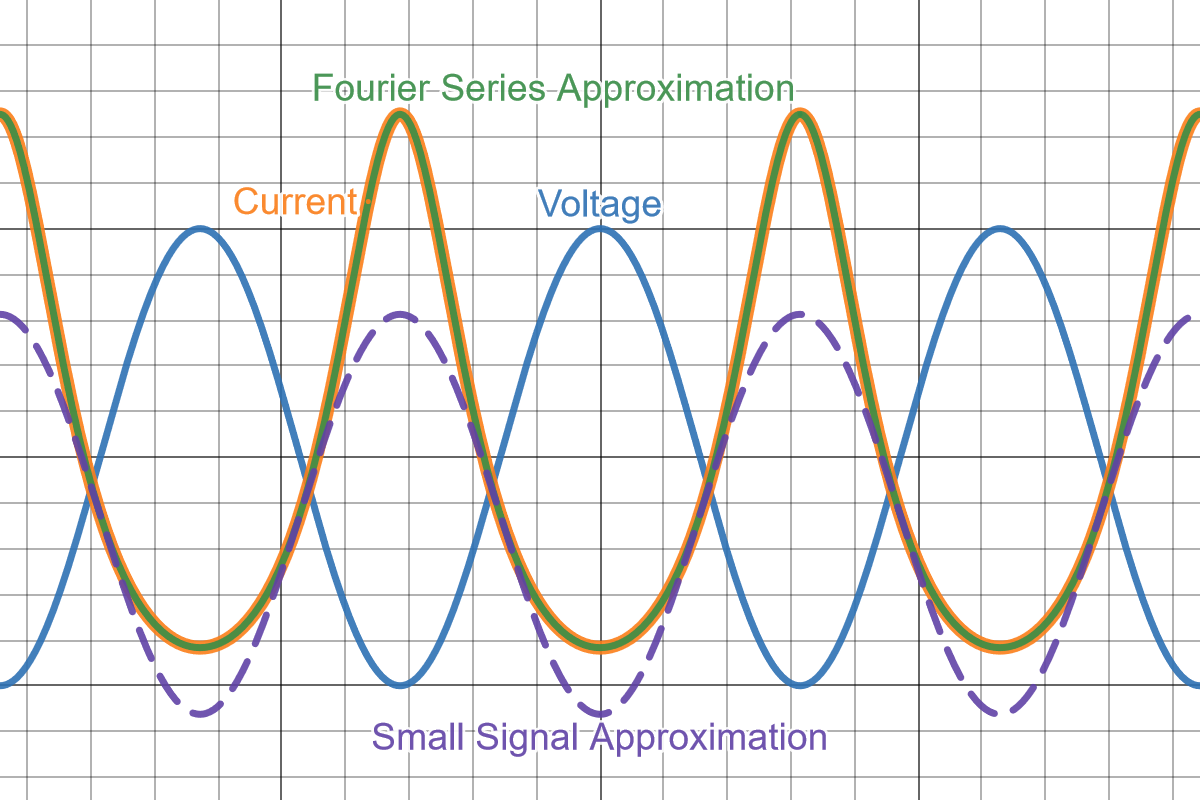
\includegraphics[width=0.5\linewidth]{figs/cpl_fourier_rect.png}
%     \caption{Fourier and small signal approximation to constant power load current.}
%     \label{fig:results}
% \end{figure}



\setcounter{section}{0}
\renewcommand\thesection{\Alph{section}}
\renewcommand\theequation{\Alph{section}.\arabic{equation}}
\section*{Appendix}

\setcounter{equation}{0}
\section{Arithmetic Series}

First, the sum of inverse squares (Basel problem) and also the sum of even squares 
\begin{IEEEeqnarray}{rCl}
	\sum_{m=1}^{\infty} \frac{1}{m^2} &=& \frac{\pi^2}{6} \\
	\sum_{m=2,4,\ldots}^{\infty} \frac{1}{m^2} &=& \sum_{m=1}^{\infty} \frac{1}{(2m)^2} = \frac{1}{4}\frac{\pi^2}{6}
\end{IEEEeqnarray}

Now, a helpful infinite sum
\begin{IEEEeqnarray}{rCl}
	\sum_{m} \frac{1}{(2m+1)^2} &=& 2\sum_{k=1,3,\ldots}^{\infty} \frac{1}{k^2} \nonumber\\
	&=& 2\left(\sum_{m=1}^{\infty} \frac{1}{m^2} - \sum_{m=2,4,\ldots}^{\infty} \frac{1}{m^2}\right) \nonumber\\
	&=& 2\left(\frac{\pi^2}{6} - \frac{1}{4}\frac{\pi^2}{6}\right) \nonumber\\
	&=& \frac{\pi^2}{4}. \label{eq:infinite_sum1}
\end{IEEEeqnarray}

For another helpful infinite sum, we start with the positive half finite sum
\begin{IEEEeqnarray}{rCl}
	\sum_{m=1}^{n}\frac{1}{4m^2-1} &=& \sum_{m=1}^{n}\frac{1}{2} \left(\frac{1}{2m-1}-\frac{1}{2m+1}\right) \nonumber\\
	&=& \frac{1}{2}\left(\sum_{m=1}^{n}\left(\frac{1}{2m-1}\right)-\sum_{m=1}^{n}\left(\frac{1}{2m+1}\right)\right) \nonumber\\
	&=& \frac{1}{2}\left(1 + \sum_{m=2}^{n}\left(\frac{1}{2m-1}\right) - \sum_{m=1}^{n-1}\left(\frac{1}{2m+1}\right) - \frac{1}{2n+1} \right)\nonumber\\
	&=& \frac{1}{2}\left(1 + \cancelRed{\sum_{p=m-1=1}^{n-1}\left(\frac{1}{2(p+1)-1}\right)} - \cancelRed{\sum_{m=1}^{n-1}\left(\frac{1}{2m+1}\right)} - \frac{1}{2n+1} \right)\nonumber\\
	&=& \frac{1}{2}\left(1 - \frac{1}{2n+1}\right).
\end{IEEEeqnarray}

We can find the positive half infinite sum by taking the limit as $n\rightarrow\infty$
\begin{IEEEeqnarray}{rCl}
	\sum_{m=1}^{\infty}\frac{1}{4m^2-1} &=& \lim_{n\rightarrow\infty} \frac{1}{2}\left(1-\frac{1}{2n+1}\right) \nonumber\\
	&=& \frac{1}{2}
\end{IEEEeqnarray}

Finally, we can find the infinite sum:
\begin{IEEEeqnarray}{rCl}
	\sum_{m} \frac{1}{4m^2-1} &=& -1 + 2\sum_{m=1}^{\infty}\frac{1}{4m^2-1} \nonumber\\
	&=& -1 + 2 \frac{1}{2} \nonumber\\
	&=& 0 \label{eq:infinite_sum2}
\end{IEEEeqnarray}

\setcounter{equation}{0}
\section{Second Appendix}




% \subsection{Pictures}

% \begin{figure}[htbp]
%     \center
%     \includegraphics[scale=0.06]{img/photo.jpg}
%     \caption{Sydney, NSW}
% \end{figure}

% \subsection{Citation}

% This is a citation\cite{Eg}.

\newpage

% ------------------------------------------------------------------------------
% Reference and Cited Works
% ------------------------------------------------------------------------------

\bibliographystyle{IEEEtran}
\begin{thebibliography}{1}

% \bibitem{leonard_2014}
% J.\@ P.\@ Leonard, ``Nonlinear Modeling Of Dc Constant Power Loads With Frequency Domain Volterra Kernels,''Florida State University, 2014.

\end{thebibliography}
% ------------------------------------------------------------------------------

\end{document}